\typeout{************************************************}
\typeout{Exercises 1.6.5 Exercises}
\typeout{************************************************}
%
\begin{exercises-subsection}{Exercises}{}{Exercises}{}{}{ez-changing-composite}
\begin{divisionexercise}{1}{}{}{ez-composite-tables-graphs-formulas}%
\hypertarget{p-510}{}%
Use the given information about various functions to answer the following questions involving composition.%
\par
\hypertarget{p-511}{}%
\leavevmode%
\begin{enumerate}[label=\alph*.]
\item\hypertarget{li-227}{}\hypertarget{p-512}{}%
Let functions $f$ and $g$ be given by the graphs in \hyperref[F-composite-ez-f]{Figure~\ref{F-composite-ez-f}} and \hyperref[F-composite-ez-g]{\ref{F-composite-ez-g}}.  An open circle means there is not a point at that location on the graph.  For instance, $f(-1) = 1$, but $f(3)$ is not defined.%
\begin{sidebyside}{2}{0}{0}{0}%
\begin{sbspanel}{0.5}%
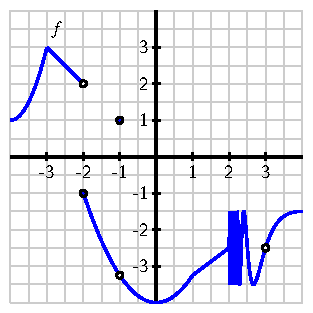
\includegraphics[width=1\linewidth]{images/composite-ez-f}
\end{sbspanel}%
\begin{sbspanel}{0.5}%
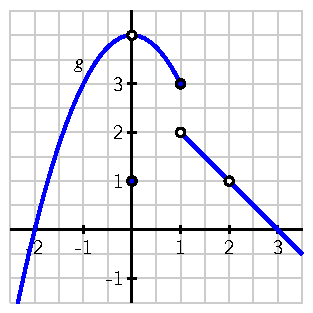
\includegraphics[width=1\linewidth]{images/composite-ez-g}
\end{sbspanel}%
\nopagebreak%
\begin{sbscaption}{0.5}%
\captionof{figure}{Plot of $y = f(x)$.\label{F-composite-ez-f}}
\end{sbscaption}%
\begin{sbscaption}{0.5}%
\captionof{figure}{Plot of $y = g(x)$.\label{F-composite-ez-g}}
\end{sbscaption}%
\end{sidebyside}%
\par
\hypertarget{p-513}{}%
Determine $f(g(1))$ and $g(f(-2))$.%
\item\hypertarget{li-228}{}\hypertarget{p-514}{}%
Again using the functions given in (a), can you determine a value of $x$ for which $g(f(x))$ is not defined?  Why or why not?%
\item\hypertarget{li-229}{}\hypertarget{p-515}{}%
Let functions $r$ and $s$ be defined by \hyperref[T-ez-composite-tables]{Table~\ref{T-ez-composite-tables}}.%
\begin{table}
\centering
\begin{tabular}{rrrrrrrrrr}
$t$&$-4$&$-3$&$-2$&$-1$&$0$&$1$&$2$&$3$&$4$\tabularnewline\hrulethin
$r(t)$&$4$&$1$&$2$&$3$&$0$&$-3$&$2$&$-1$&$-4$\tabularnewline\hrulethin
$s(t)$&$-5$&$-6$&$-7$&$-8$&$0$&$8$&$7$&$6$&$5$
\end{tabular}
\caption{Table that defines $r$ and $s$.\label{T-ez-composite-tables}}
\end{table}
\hypertarget{p-516}{}%
Determine $(s \circ r)(3)$, $(s \circ r)(-4)$, and $(s \circ r)(a)$ for one additional value of $a$ of your choice.%
\item\hypertarget{li-230}{}\hypertarget{p-517}{}%
For the functions $r$ and $s$ defined in (c), state the domain and range of each function.  For how many different values of $b$ is it possible to determine $(r \circ s)(b)$?  Explain.%
\item\hypertarget{li-231}{}\hypertarget{p-518}{}%
Let $m(u) = u^3 + 4u^2 - 5u + 1$.  Determine expressions for $m(x^2)$, $m(2+h)$, and $m(a+h)$.%
\item\hypertarget{li-232}{}\hypertarget{p-519}{}%
For the function $F(x) = 4 - 3x - x^2$, determine the most simplified expression you can find for $AV_{[2,2+h]}$.  Show your algebraic work and thinking fully.%
\end{enumerate}
%
\end{divisionexercise}%
\begin{divisionexercise}{2}{}{}{ez-composite-Dolbear-revisited}%
\hypertarget{p-522}{}%
Recall Dolbear's function that defines temperature, $F$, in Fahrenheit degrees, as a function of the number of chirps per minute, $N$, is $F = D(N) = 40 + \frac{1}{4}N$.%
\par
\hypertarget{p-523}{}%
\leavevmode%
\begin{enumerate}[label=\alph*.]
\item\hypertarget{li-233}{}\hypertarget{p-524}{}%
Solve the equation $F = 40 + \frac{1}{4}N$ for $N$ in terms of $F$.%
\item\hypertarget{li-234}{}\hypertarget{p-525}{}%
Say that $N = g(F)$ is the function you just found in (a).  What is the meaning of this function? What does it take as inputs and what does it produce as outputs?%
\item\hypertarget{li-235}{}\hypertarget{p-526}{}%
How many chirps per minute do we expect when the outsidet temperature is $82$ degrees F?  How can we express this in the notation of the function $g$?%
\item\hypertarget{li-236}{}\hypertarget{p-527}{}%
Recall that the function that converts Fahrenheit to Celcius is $C = G(F) = \frac{5}{9}(F-32)$. Solve the equation $C = \frac{5}{9}(F-32)$ for $F$ in terms of $C$.  Call the resulting function $F = p(C)$.  What is the meaning of this function?%
\item\hypertarget{li-237}{}\hypertarget{p-528}{}%
Is it possible to write the chirp-rate $N$ as a function of temperature $C$ in Celsius? That is, can we produce a function whose input is in degrees Celsius and whose output is the number of chirps per minute? If yes, do so and explain your thinking.  If not, explain why it's not possible.%
\end{enumerate}
%
\end{divisionexercise}%
\begin{divisionexercise}{3}{}{}{ez-composite-spherical-tank}%
\hypertarget{p-531}{}%
A spherical tank has radius $4$ feet.  The tank is initially empty and then begins to be filled in such a way that the height of the water rises at a constant rate of $0.4$ feet per minute.  Let $V$ be the volume of water in the tank at a given instant, and $h$ the depth of the water at the same instant; let $t$ denote the time elapsed in minutes since the tank started being filled.%
\par
\hypertarget{p-532}{}%
\leavevmode%
\begin{enumerate}[label=\alph*.]
\item\hypertarget{li-238}{}\hypertarget{p-533}{}%
Calculus can be used to show that the volume, $V$, is a function of the depth, $h$, of the water in the tank according to the function%
\begin{equation}
V = f(h) = \frac{\pi}{3} h^2(12-h)\text{.}\label{E-ez-composite-spherical-tank-V-h}
\end{equation}
What is the domain of this model?  Why?  What is the corresponding range?%
\item\hypertarget{li-239}{}\hypertarget{p-534}{}%
We are given the fact that the tank is being filled in such a way that the height of the water rises at a constant rate of $0.4$ feet per minute.  Said differently, $h$ is a function of $t$ whose average rate of change is constant.  What kind of function does this make $h = p(t)$?  Determine a formula for $p(t)$.%
\item\hypertarget{li-240}{}\hypertarget{p-535}{}%
What are the domain and range of the function $h = p(t)$?  How is this tied to the dimensions of the tank?%
\item\hypertarget{li-241}{}\hypertarget{p-536}{}%
In (a) we observed that $V$ is a function of $h$, and in (b) we found that $h$ is a function of $t$.  Use these two facts and function composition appropriately to write $V$ as a function of $t$.  Call the resulting function $V = q(t)$.%
\item\hypertarget{li-242}{}\hypertarget{p-537}{}%
What are the domain and range of the function $q$?  Why?%
\item\hypertarget{li-243}{}\hypertarget{p-538}{}%
On the provided axes, sketch accurate graphs of $h = p(t)$ and $V = q(t)$, labeling the vertical and horizontal scale on each graph appropriately.  Make your graphs as precise as you can; use a computing device to assist as needed.%
\begin{sidebyside}{2}{0}{0}{0}%
\begin{sbspanel}{0.5}%
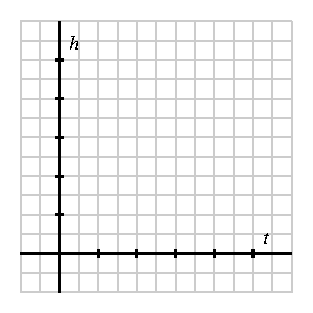
\includegraphics[width=1\linewidth]{images/tandem-h-t-blank-axes}
\end{sbspanel}%
\begin{sbspanel}{0.5}%
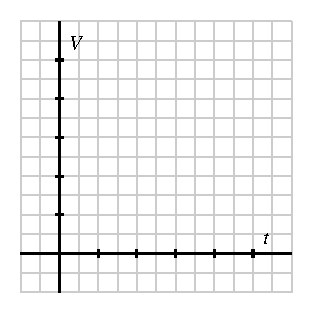
\includegraphics[width=1\linewidth]{images/tandem-V-t-blank-axes}
\end{sbspanel}%
\end{sidebyside}%
\par
\hypertarget{p-539}{}%
Why do each of the two graphs have their respective shapes?  Write at least one sentence to explain each graph; refer explicitly to the shape of the tank and other information given in the problem.%
\end{enumerate}
